\documentclass[letterpaper,10pt,conference]{ieeeconf}

\IEEEoverridecommandlockouts
\overrideIEEEmargins

\usepackage[T1]{fontenc}
\usepackage{amsmath,amssymb}
\usepackage{graphicx}
\usepackage{booktabs}
\usepackage{array}
\usepackage{multirow}
\usepackage{cite}
\usepackage{url}
\usepackage{flushend}
\usepackage{placeins}
\usepackage[hidelinks]{hyperref}

\newcommand{\etal}{et al.}
\newcommand{\method}{WarpVox}

\title{WarpVox: Observation-Guided Deformation for TSDF Map Correction after Loop Closure}

\author{Anonymous Authors}

\begin{document}
\maketitle
\thispagestyle{empty}
\pagestyle{empty}

\begin{abstract}
Loop closure retroactively changes sensor poses after their range observations
have been fused, leaving a TSDF inconsistent with the corrected trajectory.
Voxblox full reintegration restores consistency but scales with the accumulated
frame history. WarpVox instead retains bounded, timestamped surface-support
records during streaming fusion. At correction time, it uses these records and
the corrected poses to compute robust surface targets, propagates them through
one constrained ARAP solve on a coarse proxy, and transfers the warped zero set
and source-volume support into a standard Voxblox TSDF. Correction therefore
requires no historical range frames and scales with active geometry rather than
redundant observations. Across 39 Kimera-Multi and 12 KITTI loop checkpoints at
0.25 m resolution, WarpVox is the closest evaluated alternative to the
representation-matched Voxblox reintegration reference at every reported
threshold. Its F@25 differs by only 0.06 and 0.32 percentage points, while core
update time is 2.43 and 4.89 s versus 109.25 and 15.73 s, respectively. A
separate seven-checkpoint native-mesh study improves mean F@50 by 5.83
percentage points over Kimera-PGMO while running $9.05\times$ faster on average
and up to $11.31\times$ faster. On one SplaTAM sequence, a geometry-only
extension reaches 40.59 F@50 versus 41.01 for a corrected-pose rebuild, with
approximately 21 s rather than 2 h of update time. WarpVox creates no new
surface adjacency; missing or topologically corrupted geometry remains outside
its scope.
\end{abstract}

\begin{figure*}[t]
\centering
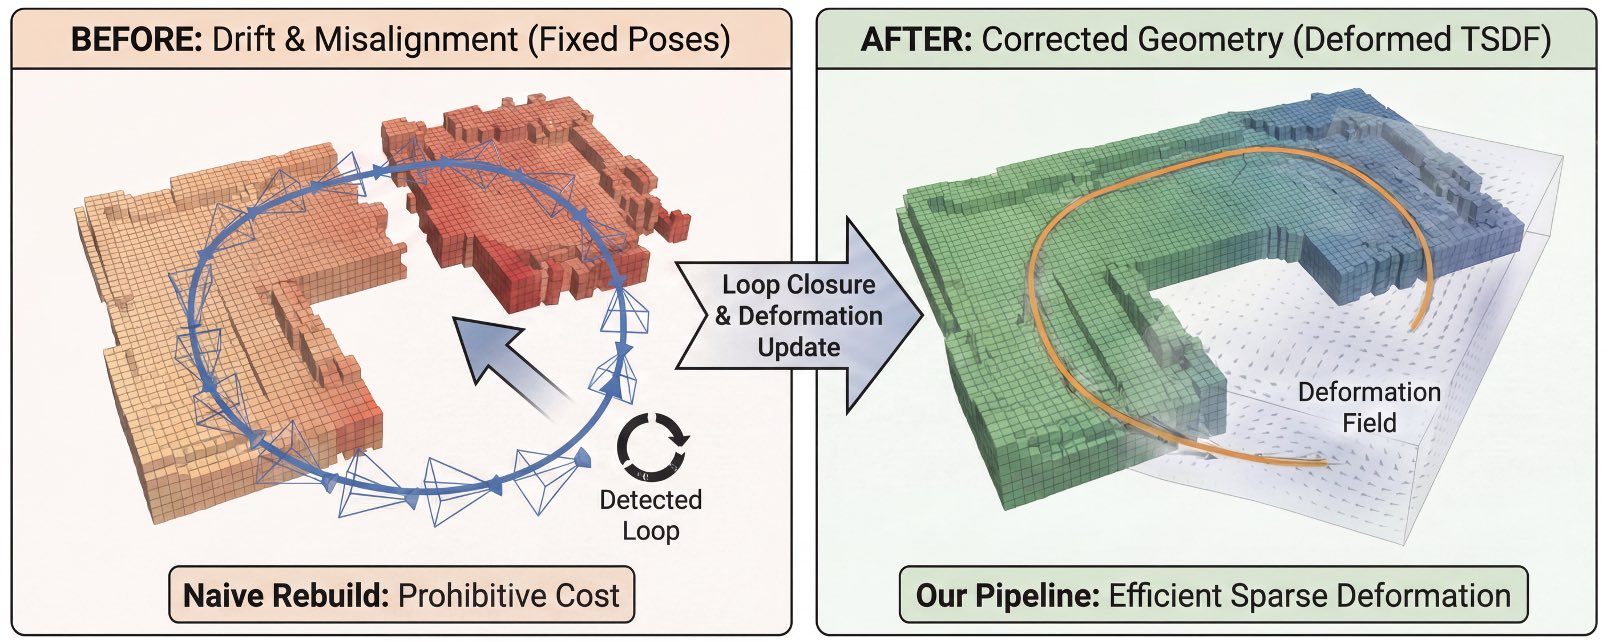
\includegraphics[width=0.92\textwidth]{Figures/teaser_v1.jpg}
\caption{\textbf{WarpVox corrects a TSDF after loop closure without
reintegrating historical measurements.} The pre-correction map is locally
coherent but globally inconsistent with the corrected trajectory. WarpVox
computes surface targets from retained sensor-frame support, deforms the
surface once, and reconstructs a corrected TSDF.}
\label{fig:teaser}
\end{figure*}

% PaperCept keywords: Dense mapping; loop closure; TSDF;
% non-rigid deformation; SLAM.

\section{Introduction}
\label{sec:intro}

Dense 3D maps support navigation, manipulation, and scene understanding in robotics and augmented reality. TSDF methods~\cite{10.1145/3596711.3596726,newcombe2011kinectfusion} integrate range measurements incrementally, while sparse data structures~\cite{10.1145/2508363.2508374,Oleynikova_2017,vizzo2022vdbfusion} make large-scale onboard mapping practical.

These systems accept sensor poses from an external SLAM front-end but cannot revise measurements already fused into the map. Loop closure and pose-graph optimization~\cite{Campos_2021,5979949} retroactively correct the trajectory, leaving the TSDF in the old world geometry and therefore inconsistent with the corrected poses (Fig.~\ref{fig:teaser}).

\vspace{1mm}\noindent\textit{The map rebuild bottleneck.}
The standard remedy is to discard the map and reintegrate all $N$ range frames with corrected poses~\cite{Cramariuc_2023,rosinol2021kimeraslamspatialperception}. Its $O(N|\Omega|)$ cost, for $|\Omega|$ measurements per frame, must be paid again after every loop closure and can take minutes on long sessions.

\vspace{1mm}\noindent\textit{Why existing solutions fall short.}
Submap methods such as Voxgraph~\cite{reijgwart2020voxgraph} and FlashFusion~\cite{han2018flashfusion} apply rigid per-submap transforms but leave intra-submap drift uncorrected. Non-rigid surfel SLAM~\cite{whelan2016elasticfusion} is self-contained rather than an external TSDF correction interface, while neural implicit approaches~\cite{sucar2021imap,zhu2022niceslam,liso2024loopyslam,bruns2024neuralgraphmap} either lack loop closure or require expensive re-optimization.

\vspace{1mm}\noindent\textit{Observation invariance: the key insight.}
A calibrated surface sample expressed in its sensor frame is unchanged by a later world-frame pose correction. WarpVox therefore retains a bounded set of such samples with their acquisition times and surface support. Re-expressing them with corrected poses yields corrected world-space targets, so loop correction consumes bounded records rather than the historical range stream.

\vspace{1mm}\noindent\textit{Our approach.}
WarpVox uses four stages: (i)~associate bounded sensor-frame evidence with the pre-correction surface, (ii)~compute robust targets from corrected poses, (iii)~propagate sparse displacements through a single event-level ARAP optimization~\cite{ARAP_modeling:2007} on a QEM proxy, and (iv)~reconstruct a TSDF whose zero set follows the warped surface while support and confidence follow the source volume. The last step matters because a surface-only conversion would mark unsupported space as observed. Once the records are maintained by the mapper, correction scales with active surface and volume rather than accumulated frames.

\vspace{1mm}\noindent\textit{Contributions.}
\begin{itemize}
    \item We formulate loop-closure map correction from bounded observation-support records, decoupling correction from accumulated raw frames.
    \item We combine observation-derived targets, a single event-level proxy deformation, and source-supported reconstruction to return a Voxblox-compatible TSDF that replaces the active volume and supports continued fusion across subsequent loop closures.
    \item We evaluate against full reintegration and mapping baselines over 51 checkpoints, separately compare final-state correction with Kimera-PGMO over ten complete Kimera-Multi bags, and extend the target mechanism to Gaussian primitives.
\end{itemize}
% Additional RA-L material is integrated into the main introduction.

\section{Related Work}
\label{sec:related}

\vspace{1mm}\noindent\textit{Volumetric SLAM and dense mapping.}
The seminal work of Curless and Levoy~\cite{10.1145/3596711.3596726} established TSDF integration as the standard paradigm for dense surface reconstruction from range data. KinectFusion~\cite{newcombe2011kinectfusion} demonstrated real-time volumetric fusion on GPU by coupling ICP-based tracking with TSDF integration into a fixed-size voxel grid. Spatial hashing~\cite{10.1145/2508363.2508374} extended this to unbounded scenes by allocating voxel blocks on demand. Voxblox~\cite{Oleynikova_2017} introduced an efficient incremental SDF mapping library designed for on-board deployment on MAVs, consuming poses from any external odometry source. VDBFusion~\cite{vizzo2022vdbfusion} provides a flexible alternative based on the OpenVDB hierarchical volume format. A common design assumption across all these systems is that the input trajectory is fixed; none provides a mechanism for updating the volumetric map when the trajectory is retroactively corrected by a pose-graph SLAM back-end.

\vspace{1mm}\noindent\textit{Loop closure in dense SLAM.}
Kintinuous~\cite{whelan2015kintinuous} addressed large-scale dense mapping by maintaining a sliding TSDF window and extracting point cloud slices as the camera moves; loop closure is handled by aligning cloud slices with a deformation graph, but only at the submap boundary level. ElasticFusion~\cite{whelan2016elasticfusion} represents the scene as a surfel map and performs frequent local non-rigid deformations using an embedded deformation graph, enabling real-time loop closure within its own tracking system. However, it is a self-contained SLAM system designed for room-scale environments, and its deformation mechanism is not directly applicable to an external TSDF receiving discrete pose-graph corrections. FlashFusion~\cite{han2018flashfusion} achieves real-time globally consistent reconstruction on CPU via rigid submaps and boundary reintegration. Voxgraph~\cite{reijgwart2020voxgraph} jointly optimizes a pose graph over SDF submaps, but likewise applies rigid per-submap corrections. WarpVox instead deforms an extracted surface with spatially varying targets and reconstructs a single corrected TSDF without decomposing the map into rigid submaps.

\vspace{1mm}\noindent\textit{Non-rigid deformation for 3D reconstruction.}
As-Rigid-As-Possible (ARAP) surface modeling~\cite{ARAP_modeling:2007} minimizes local rigidity distortion subject to positional constraints. Sumner \etal~\cite{10.1145/1276377.1276478} introduced embedded deformation graphs as sparse controls for arbitrary shapes. DynamicFusion~\cite{7298631}, KillingFusion~\cite{slavcheva2017killingfusion}, and VolumeDeform~\cite{innmann2016volumedeform} estimate non-rigid scene motion through continuous frame-to-frame tracking. Our setting instead receives a discrete trajectory correction for a static map. WarpVox uses the corrected poses and vertex--observation associations to compute surface targets, then propagates them with a single ARAP solve on a QEM proxy.

\vspace{1mm}\noindent\textit{Neural and Gaussian maps.}
iMAP~\cite{sucar2021imap}, NICE-SLAM~\cite{zhu2022niceslam}, and NGEL-SLAM~\cite{cui2023ngelslam} optimize neural scene representations, while Loopy-SLAM~\cite{liso2024loopyslam} couples loop closure to neural-map re-optimization. Neural Graph Map~\cite{bruns2024neuralgraphmap} instead anchors local fields to pose-graph nodes. Three-dimensional Gaussian splatting (3DGS) targets high-quality real-time rendering~\cite{kerbl2023gaussians}; SplaTAM~\cite{keetha2024splatam} uses differentiable rendering for dense RGB-D SLAM, and LoopSplat~\cite{zhu2025loopsplat} restores global consistency by rigidly aligning Gaussian submaps. These representations are effective for rendering, but they do not natively provide the signed-distance and observed-free-space structure used for obstacle-distance mapping. WarpVox primarily targets TSDF/ESDF robotics pipelines, while our geometry-only Gaussian experiment tests whether its observation-derived targets transfer beyond voxel grids.

% Additional RA-L material is integrated into the main related-work section.

\section{Method}
\label{sec:method}

\noindent\textbf{Assumptions.}
Following the local-consistency assumption of
Voxgraph~\cite{reijgwart2020voxgraph}, we assume that TSDF fusion under the
drifted pre-correction trajectory remains locally valid: surface geometry and
connectivity are coherent in local neighborhoods although the map is globally
inconsistent. WarpVox corrects this global inconsistency after loop closure;
severely noisy or topologically corrupted source maps are outside its scope.

\subsection{Problem and Streaming State}

Let $T_i^- ,T_i^+\in SE(3)$ map sensor frame $S_i$ to the world frame before
and after trajectory correction. The map built with $\{T_i^-\}$ consists of a
TSDF $\Phi^-$, its weight field $w^-$, voxel size $s$, and truncation distance
$\tau$. Marching Cubes (MC)~\cite{10.1145/37402.37422} extracts the source
surface $\mathcal M^-=(V^-,F)$.

During fusion, WarpVox retains timestamped sensor-frame surface samples in a
bounded state indexed by the active TSDF cells $\mathcal A$:
\begin{equation}
\mathcal S=\{\mathcal S_c\}_{c\in\mathcal A},
\qquad |\mathcal S_c|\le n_c.
\label{eq:streaming_state}
\end{equation}
After surface extraction, each vertex queries a fixed neighboring-cell stencil
and applies the geometric validation below. We write this Stage-1 resolution as
\begin{equation}
\begin{aligned}
\mathcal O&=\mathcal R(\mathcal M^-,\{T_i^-\},\mathcal S),\\
\mathcal O_j&=\{(t_i,m_{ij},\alpha_{ij})\},
\qquad |\mathcal O_j|\le n_v,
\end{aligned}
\label{eq:resolved_records}
\end{equation}
where $m_{ij}$ is expressed in $S_i$ and $\alpha_{ij}\in[0,1]$ is the
effective reliability of the retained association. Records are matched by
acquisition time rather than trajectory row index. Thus the online state is
cell-indexed, while the correction backend receives bounded vertex-indexed
records without retaining the range stream:
\begin{equation}
(\Phi^-,w^-,\mathcal M^-,\{T_i^+\},\mathcal O)
\longmapsto (\Phi^+,w^+).
\label{eq:contract}
\end{equation}
The warped mesh is intermediate; $(\Phi^+,w^+)$ is the returned
Voxblox-compatible TSDF.

\begin{figure}[t]
  \centering
  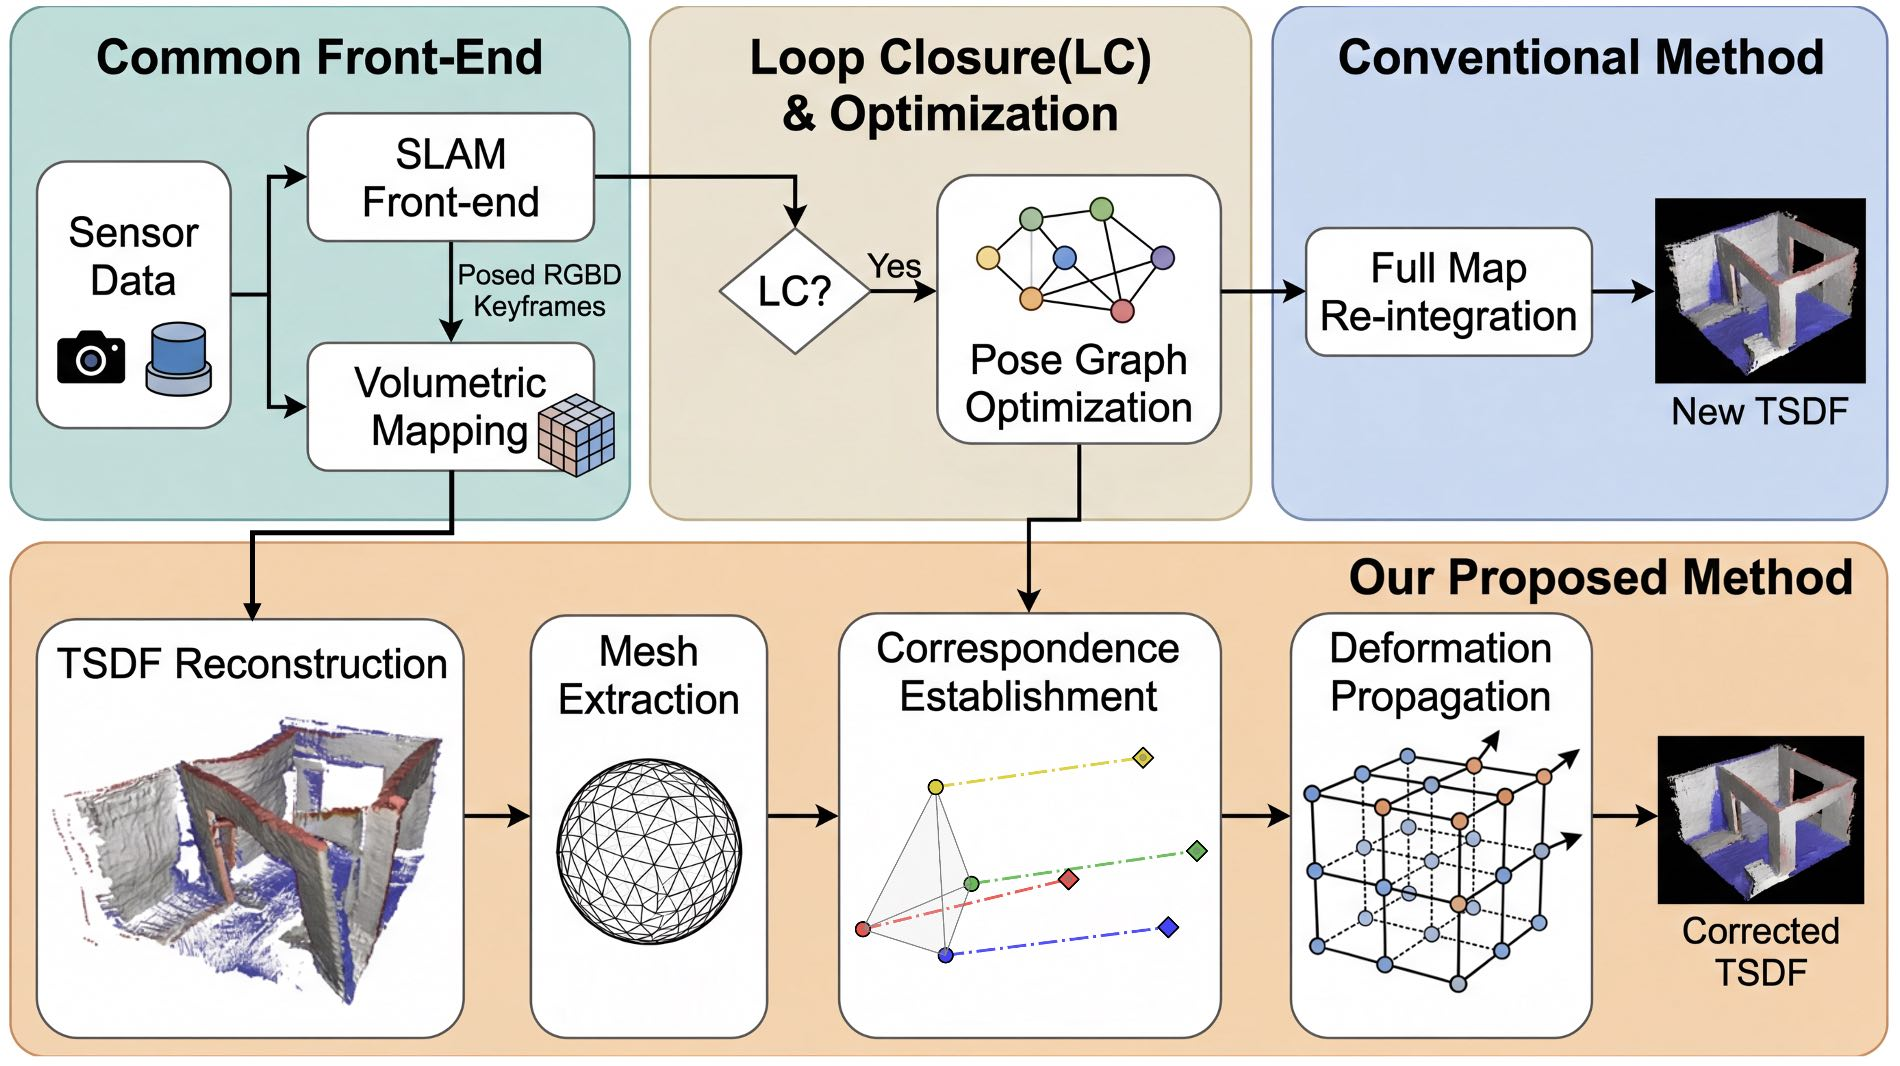
\includegraphics[width=\linewidth]{Figures/pipeline_v5.jpg}
  \caption{WarpVox retains bounded observation support during fusion, resolves
  surface observations after extraction, computes corrected targets from the
  revised trajectory, performs one event-level proxy deformation, and transfers
  source-volume support to the corrected TSDF.}
  \label{fig:pipeline}
\end{figure}

\subsection{Observation Association and Surface Targets}

For RGB-D, pixel $\bar u=[u,v,1]^\top$ with measured z-depth $z_{ij}$ defines
the invariant sensor-frame sample
\begin{equation}
m_{ij}=z_{ij}K^{-1}\bar u,
\qquad
\widetilde m_{ij}=[m_{ij}^\top,1]^\top.
\label{eq:sensor_sample}
\end{equation}
The pre-correction pose projects source vertex $v_j^-$ into frame $i$.
Candidate observations must agree in depth, three-dimensional position, and
viewing direction. Let $n_j^-$ be the source normal, $r_{ij}^-$ the unit
viewing direction in the pre-correction world frame, and $z_{ij}^{\rm proj}$
the projected vertex depth. Define
\begin{equation}
\begin{aligned}
e^g_{ij}
&=\left\|[T_i^-\widetilde m_{ij}]_{1:3}-v_j^-\right\|,\\
e^z_{ij}
&=z_{ij}^{\rm proj}-z_{ij},\\
g_{ij}
&=\left|(n_j^-)^\top r_{ij}^-\right|.
\end{aligned}
\label{eq:association_residuals}
\end{equation}
The effective association reliability is
\begin{equation}
\alpha_{ij}=
\exp\!\left(-\frac{e^g_{ij}}{\sigma_g}\right)
\exp\!\left(-\frac{|e^z_{ij}|}{\sigma_z}\right)
\frac{g_{ij}}{1+z_{ij}^{\rm proj}/z_0},
\label{eq:association_weight}
\end{equation}
subject to a depth-dependent geometric gate and a minimum reliability. LiDAR
uses the analogous construction with spherical projection and radial range.
This is geometric support rather than exact voxel-integration provenance. The
$z_0$ term ranks distant samples during capped association; a separate range
factor below models target reliability after an association has been retained.

After loop closure, each timestamp selects the corresponding corrected pose.
For a missing interior pose, translation is interpolated linearly and rotation
by SLERP over a bounded gap~\cite{shoemake1985slerp}. The invariant sample then
defines the corrected candidate
\begin{equation}
q_{ij}^+=\left[T_i^+\widetilde m_{ij}\right]_{1:3}.
\label{eq:corrected_target}
\end{equation}
This candidate is exact when the static-scene association, calibration, and
corrected pose are valid. Let $\mathcal J_j$ index $\mathcal O_j$, and let
$\rho_{ij}$ be modality-native range, with $\rho_{ij}=z_{ij}$ for RGB-D and
$\rho_{ij}=\|m_{ij}\|$ for LiDAR. We first compute
\begin{equation}
\omega_{ij}=\frac{\alpha_{ij}}{1+\rho_{ij}/\rho_t},
\qquad
\bar q_j=
\frac{\sum_{i\in\mathcal J_j}\omega_{ij}q_{ij}^+}
     {\sum_{i\in\mathcal J_j}\omega_{ij}}.
\label{eq:target_initial}
\end{equation}
The reliability-weighted center is paired with an unweighted median residual
scale so that one high-weight candidate cannot determine both the estimate and
its rejection threshold:
\begin{equation}
\begin{aligned}
\theta_j&=\max\!\left(
\epsilon_t,
\kappa_t\operatorname*{median}_{k\in\mathcal J_j}
\|q_{kj}^+-\bar q_j\|\right),\\
I_j&=\left\{i\in\mathcal J_j:
\|q_{ij}^+-\bar q_j\|\le\theta_j\right\}.
\end{aligned}
\label{eq:target_inliers}
\end{equation}
When fewer than three candidates are available, $I_j=\mathcal J_j$. The final
target and its observable dispersion are
\begin{equation}
v_j^*=
\frac{\sum_{i\in I_j}\omega_{ij}q_{ij}^+}
     {\sum_{i\in I_j}\omega_{ij}},
\qquad
\sigma_j^2=
\frac{\sum_{i\in I_j}\omega_{ij}\|q_{ij}^+-v_j^*\|^2}
     {\sum_{i\in I_j}\omega_{ij}}.
\label{eq:target}
\end{equation}
Only targets passing fixed support and dispersion tests become controls. The
dispersion measures agreement among retained candidates but cannot detect a
mutually consistent yet incorrect association.

\subsection{Event-Level Surface Deformation}

The deformation stage propagates observation-derived motion; it does not infer
correction from shape alone. Let $d_j=v_j^*-v_j^-$ denote an accepted control
displacement. A component-aware local predictor and a median--MAD test reject
isolated displacements before coarsening.

Component-separated spatial clustering~\cite{rossignac1993vertexclustering}
constructs a triangular proxy $\mathcal P^-=(P^-,F_P)$ and selects one QEM
representative~\cite{garland1997qem} per occupied cell. Let
$\pi:V^-\rightarrow P^-$ map source vertices to representatives and
$\mathcal K_a=\{j:\pi(j)=a\}$ collect accepted controls assigned to proxy
vertex $a$. For $\mathcal K_a\neq\emptyset$, the initial proxy displacement and
target are
\begin{equation}
\bar d_a=\frac{1}{|\mathcal K_a|}\sum_{j\in\mathcal K_a}d_j,
\qquad
p_a^{(0)}=p_a^-+\bar d_a.
\label{eq:proxy_initial_target}
\end{equation}
A local-rigid consensus then validates measured proxy targets and supplies
motion where direct support is absent. Weighted orthogonal-Procrustes
fits~\cite{schoenemann1966procrustes} with Welsch
reweighting~\cite{yao2020welsch} predict the local motion; a measured target is
replaced only when it is a gross outlier and a strict same-component majority
supports the replacement. Components without accepted controls inherit a
robust nearby motion through three spatially separated synthetic anchors. Let
$\{p_a^*:a\in\mathcal C_P\}$ denote the resulting accepted or synthesized
proxy targets.

WarpVox performs one event-level proxy ARAP
optimization~\cite{ARAP_modeling:2007,
10.1007/978-3-662-05105-4_2,libigl}:
\begin{equation}
\begin{aligned}
\min_{P^+,\{R_a\in SO(3)\}}\quad
&\frac{1}{2}\sum_{a=1}^{|P^-|}
\sum_{b\in\mathcal N_P(a)}c_{ab}\\[-1mm]
&\left\|(p_a^+-p_b^+)-R_a(p_a^--p_b^-)\right\|^2,\\
\text{s.t.}\quad
&p_a^+=p_a^*,\qquad a\in\mathcal C_P .
\end{aligned}
\label{eq:arap}
\end{equation}
Here $\mathcal N_P(a)$ is the one-ring neighborhood induced by $F_P$, and
$c_{ab}=c_{ba}$ are symmetric cotangent-derived weights; the factor $1/2$
removes double counting. Reliability screening and local consensus decide which
controls survive and where they lie. Once accepted, controls are imposed
exactly so that ARAP does not attenuate the supplied trajectory correction. The
standard local--global iterations solve this single event-level optimization.

Proxy displacement is transferred to $V^-$ by topology-local interpolation. A
local bounded-distortion pass~\cite{sorkine2004laplacian,aigerman2013bounded}
harmonically repairs isolated failures and omits only faces that remain invalid
under fixed dimensionless tests. The retained source and warped surfaces
therefore satisfy
\begin{equation}
\bar{\mathcal M}^-=(\bar V^-,\bar F),
\qquad
\mathcal M^+=(\bar V^+,\bar F),
\qquad
\bar F\subseteq F.
\label{eq:retained_topology}
\end{equation}
Deformation accuracy is therefore governed by target correctness and surface
coverage; neither is independently certifiable without stronger scene
assumptions.

\subsection{Source-Supported TSDF Reconstruction}

The warped surface supplies the corrected zero set~\cite{sussman1999redistancing},
while the source TSDF supplies observed-space semantics. For output voxel center
$x$, a closest-triangle query~\cite{10.1145/2601097.2601199} on $\mathcal M^+$
returns face $f$, closest point $q^+$, and barycentric coordinates $\beta$.
Shared face indices locate the corresponding source point
\begin{equation}
q^-=\sum_{k\in f}\beta_k\bar v_k^-.
\label{eq:source_correspondence}
\end{equation}
Let
\begin{equation}
R_f^\pm=
\begin{bmatrix}
t_{f,1}^\pm & t_{f,2}^\pm & n_f^\pm
\end{bmatrix}\in SO(3)
\label{eq:triangle_frames}
\end{equation}
be consistently oriented orthonormal frames of the corresponding source and
warped triangles. The first tangent follows the same indexed edge and
$t_{f,2}^\pm=n_f^\pm\times t_{f,1}^\pm$. A piecewise local-rigid pullback,
motivated by deformation transfer~\cite{sumner2004deformationtransfer}, maps
$x$ to the source volume:
\begin{equation}
\Psi_f(x)=q^-+R_f^-(R_f^+)^\top(x-q^+),
\qquad x^-=\Psi_f(x).
\label{eq:inverse_map}
\end{equation}
This preserves tangential and normal offsets relative to the corresponding
triangles. With trilinear source samples $\widetilde\Phi^-$ and
$\widetilde w^-$, define
\begin{equation}
\begin{aligned}
r^+(x)&=\|x-q^+\|,\qquad d^+(x)=\min\!\left(\tau,r^+(x)\right),\\
\Omega_{\rm tr}&=\left\{x:\widetilde w^-(\Psi_f(x))>0\right\}.
\end{aligned}
\label{eq:transferred_support}
\end{equation}

Let $\Omega_{\rm fb}\subseteq\mathbb R^3\setminus\Omega_{\rm tr}$ contain
bounded unsupported interpolation holes connected to $\Omega_{\rm tr}$ but not
incident to an open mesh boundary. Its finite fallback weight is
\begin{equation}
w_{\rm fb}(x)=
\begin{cases}
1, & r^+(x)\le0.5s,\\
(1.5s-r^+(x))/s, & 0.5s<r^+(x)\le1.5s,\\
0, & r^+(x)>1.5s.
\end{cases}
\label{eq:fallback_weight}
\end{equation}
The warped normal is oriented to preserve the source TSDF sign convention, so
\begin{equation}
s_f^+(x)=\operatorname{sgn}\!\left((x-q^+)^\top n_f^+\right).
\label{eq:fallback_sign}
\end{equation}
Define $\Omega^+=\Omega_{\rm tr}\cup\Omega_{\rm fb}$ and
$\Phi^+:\Omega^+\rightarrow[-\tau,\tau]$ by
\begin{equation}
\Phi^+(x)=
\begin{cases}
\operatorname{sgn}\!\left(\widetilde\Phi^-(\Psi_f(x))\right)d^+(x),
& x\in\Omega_{\rm tr},\\
s_f^+(x)d^+(x),
& x\in\Omega_{\rm fb}.
\end{cases}
\label{eq:hybrid_tsdf}
\end{equation}
The output weight is
\begin{equation}
w^+(x)=
\begin{cases}
\widetilde w^-(\Psi_f(x)), & x\in\Omega_{\rm tr},\\
w_{\rm fb}(x), & x\in\Omega_{\rm fb},\\
0, & \text{otherwise}.
\end{cases}
\label{eq:hybrid_weight}
\end{equation}
Any fallback extension that introduces a new sign crossing is rejected. Outside
$\Omega^+$, zero weight makes the stored distance immaterial. The resulting
$(\Phi^+,w^+)$ is serialized in the native Voxblox TSDF format; its MC mesh is
used only for visualization and evaluation.

\subsection{Complexity and Scope}

Let $A=|\mathcal A|$, $P=|P^-|$, and $X^+$ be the numbers of active support
cells, proxy vertices, and allocated output voxels. At fixed resolution, MC
produces a constant number of surface elements per active cell, so
$|V^-|=O(A)$. The streaming and resolved correction states satisfy
\begin{equation}
S_{\rm stream}=O(n_cA),
\qquad
S_{\rm corr}=O(n_vA).
\label{eq:state_complexity}
\end{equation}
Because each source vertex queries a fixed stencil, association resolution and
target aggregation require $O((n_c+n_v)A)$. The complete correction cost is
\begin{equation}
\begin{aligned}
C_{\rm corr}={}&O((n_c+n_v)A)+C_{\rm ARAP}(P,F_P)\\
&+C_{\rm vol}(X^+,\bar F),
\end{aligned}
\label{eq:complexity}
\end{equation}
where $C_{\rm vol}$ is the accelerated closest-triangle reconstruction cost. In
the streaming realization, accumulated frame count $N$ does not appear:
bounded support replaces history-dependent replay, while the remaining work
follows the active surface, proxy, and output volume.

\section{Experiments}
\label{sec:experiments}

\subsection{Evaluation Protocol}

We evaluate 39 RGB-D loop-closure cases from 18 Kimera-Multi
sequences~\cite{tian23arxiv_kimeramultiexperiments} and 12 LiDAR cases from
six KITTI sequences~\cite{Geiger2013IJRR}. Every method reconstructs the same
temporal interval and uses the same GT: a 5 m tube around the official
Kimera-Multi trajectory or GT-registered KITTI points within the mapper's 25 m
ray range. Predictions outside the GT frame are aligned by a RANSAC--Umeyama
$\mathrm{Sim}(3)$ fitted only to timestamp-matched trajectory positions; no
mesh-to-GT registration is used. Inputs are replayed offline, but map updates
remain sequential: each corrected TSDF replaces the active Voxblox volume and
fusion continues to the next loop closure.

\noindent\textbf{Baselines.}
Uncorrected TSDF uses the pre-correction trajectory. Open3D~\cite{zhou2018open3dmodernlibrary3d}
and Wavemap~\cite{reijgwart2023wavemap} replay corrected poses into an
independent TSDF and a wavelet occupancy map, respectively; Voxgraph
~\cite{reijgwart2020voxgraph} optimizes rigid TSDF submaps. Voxblox
reintegration~\cite{Oleynikova_2017} is the representation-matched reference.
WarpVox instead uses the uncorrected TSDF, sensor-frame support, and the
pre/post-correction trajectories. For deterministic offline evaluation, Stage
1 is reproduced by replaying only recorded keyframes after the pre-mesh is
available; online, the same associations accumulate as keyframes arrive.

We compute precision and recall by bidirectional nearest-neighbour tests and
report F@10/25/50 at 0.10/0.25/0.50 m. All methods share each case's crop,
spatial region, two-million-point sample, random seed, and thresholds. Main
TSDF experiments use 0.25 m voxels and 1.0 m truncation; Wavemap uses a matched
0.25 m finest level. Core times are measured on an AMD Ryzen 7 9700X with 64 GB
RAM from in-memory inputs; bag reading, disk I/O, serialization, visualization,
evaluation, and evaluation-only Marching Cubes are excluded.

\subsection{Reconstruction Fidelity and Update Cost}

Table~\ref{tab:broad_main} gives the uniform 0.25 m comparison. WarpVox is
the closest method to Voxblox reintegration at every threshold, with absolute
deviations below 0.27 pp on Kimera-Multi and 0.39 pp on KITTI, and has the best
F@25 and F@50 among non-reference methods on both datasets.

\begin{table}[t]
\centering
\caption{\textbf{Reconstruction accuracy and mean core update time at
0.25 m.} F-scores are percentages; lower time is better.}
\label{tab:broad_main}
\scriptsize
\setlength{\tabcolsep}{2.1pt}
\begin{tabular}{llrrrr}
\toprule
Data & Method & F@10 & F@25 & F@50 & Core (s) \\
\midrule
\multirow{6}{*}{K-Multi (39)}
 & Uncorrected TSDF & 7.00 & 19.29 & 34.91 & -- \\
 & Open3D & 8.13 & 22.94 & 41.30 & -- \\
 & Voxgraph & 8.27 & 22.78 & 39.49 & 5.54 \\
 & Wavemap & 1.73 & 11.54 & 30.91 & 8.32 \\
 & Voxblox reintegration & 10.93 & 28.71 & \textbf{48.67} & 109.25 \\
 & \textbf{WarpVox} & \textbf{11.13} & \textbf{28.77} & 48.40 & 2.43 \\
\midrule
\multirow{6}{*}{KITTI (12)}
 & Uncorrected TSDF & 7.13 & 27.91 & 49.22 & -- \\
 & Open3D & \textbf{13.50} & 38.58 & 61.02 & -- \\
 & Voxgraph & 9.38 & 31.89 & 52.49 & 4.53 \\
 & Wavemap & 5.23 & 33.10 & 62.55 & 2.68 \\
 & Voxblox reintegration & 13.21 & \textbf{44.29} & \textbf{67.45} & 15.73 \\
 & \textbf{WarpVox} & 13.00 & 43.98 & 67.06 & 4.89 \\
\bottomrule
\end{tabular}
\vspace{1pt}

\parbox{\columnwidth}{\scriptsize Times for unchanged baselines are retained
from their canonical runs; WarpVox is remeasured with the final implementation.}
\end{table}

WarpVox is $45.1\times$ faster than reintegration on Kimera-Multi and
$3.22\times$ on KITTI. The smaller KITTI gain follows from cheap sparse-LiDAR
replay versus WarpVox's larger active surface and output volume, while its TSDF
remains the closest alternative to the reference.

Table~\ref{tab:runtime_breakdown} separates the four stages. For
Kimera-Multi, the unchanged Stage 1--2 measurements are combined with the
remeasured final Stage 3--4 implementation. For KITTI, all four stages are
remeasured; its Stage 3 mean comprises 2.457 s of ARAP deformation and
0.148 s of topology processing.

\begin{table}[t]
\centering
\caption{\textbf{Mean WarpVox core-time breakdown in seconds.}}
\label{tab:runtime_breakdown}
\scriptsize
\setlength{\tabcolsep}{2.3pt}
\begin{tabular}{lrrrrr}
\toprule
Setting & Stage 1 & Stage 2 & Stage 3 & Stage 4 & Total \\
\midrule
K-Multi, 25 cm (39) & 0.460 & 0.400 & 1.375 & 0.190 & 2.425 \\
KITTI, 25 cm (12)   & 0.310 & 0.069 & 2.605 & 1.907 & 4.890 \\
K-Multi, 10 cm (11) & 4.138 & 0.250 & 5.052 & 0.993 & 10.432 \\
\bottomrule
\end{tabular}
\vspace{1pt}

\parbox{\columnwidth}{\scriptsize Stage 1: association; Stage 2: target
aggregation; Stage 3: deformation and topology processing; Stage 4: TSDF
reconstruction. Component means are rounded independently.}
\end{table}

As a resolution-transfer check, the same 11 Kimera-Multi cases reconstructed
at 0.10 m obtain F@10/25/50 of 17.13/39.76/57.83 with WarpVox, compared with
17.21/39.68/57.12 for Voxblox reintegration. WarpVox requires 10.432 s of
core computation versus 192.548 s for reintegration, an $18.5\times$
reduction. The close quantitative agreement is complemented by the
qualitative comparisons in Fig.~\ref{fig:qualitative_ral}.

\begin{figure*}[t]
\centering
\setlength{\tabcolsep}{0pt}
\renewcommand{\arraystretch}{0.2}
\newcommand{\qa}[1]{\includegraphics[width=.245\linewidth,trim=150 150 150 150,clip]{#1}}
\newcommand{\qb}[1]{\includegraphics[width=.245\linewidth,trim=250 70 250 70,clip]{#1}}
\newcommand{\qc}[1]{\includegraphics[width=.245\linewidth,trim=200 20 200 20,clip]{#1}}
\newcommand{\qd}[1]{\includegraphics[width=.245\linewidth,trim=100 20 100 20,clip]{#1}}
\begin{tabular}{cccc}
\qa{Figures/qualitative/5_voxblox_pre.png} &
\qa{Figures/qualitative/5_voxblox_post.png} &
\qa{Figures/qualitative/5_voxgraph_post_sep.png} &
\qa{Figures/qualitative/5_warped_tsdf.png} \\[2pt]
\qb{Figures/qualitative/28_voxblox_pre.png} &
\qb{Figures/qualitative/28_voxblox_post.png} &
\qb{Figures/qualitative/28_voxgraph_post_sep.png} &
\qb{Figures/qualitative/28_warped_tsdf.png} \\[2pt]
\qc{Figures/qualitative/40_voxblox_pre.png} &
\qc{Figures/qualitative/40_voxblox_post.png} &
\qc{Figures/qualitative/40_voxgraph_post_sep.png} &
\qc{Figures/qualitative/40_warped_tsdf.png} \\[2pt]
\qd{Figures/qualitative/35_voxblox_pre.png} &
\qd{Figures/qualitative/35_voxblox_post.png} &
\qd{Figures/qualitative/35_voxgraph_post_sep.png} &
\qd{Figures/qualitative/35_warped_tsdf.png} \\[4pt]
\qc{Figures/qualitative/76_voxblox_pre.png} &
\qc{Figures/qualitative/76_voxblox_post.png} &
\qc{Figures/qualitative/76_voxgraph_post_sep.png} &
\qc{Figures/qualitative/76_warped_tsdf.png} \\[2pt]
\qd{Figures/qualitative/77_voxblox_pre.png} &
\qd{Figures/qualitative/77_voxblox_post.png} &
\qd{Figures/qualitative/77_voxgraph_post_sep.png} &
\qd{Figures/qualitative/77_warped_tsdf.png} \\[2pt]
\small Voxblox$_{\mathrm{Pre}}$ &
\small Voxblox reintegration &
\small Voxgraph &
\small \textbf{WarpVox}
\end{tabular}
\caption{\textbf{Qualitative reconstruction comparison at 0.25 m.} Four
Kimera-Multi loop-closure cases are shown in the top four rows and two KITTI
cases in the bottom two rows; each row uses the same view across methods.}
\label{fig:qualitative_ral}
\end{figure*}

\subsection{Event-Triggered Comparison with Kimera-PGMO}

Kimera-PGMO continuously maintains a MeshFrontend deformation graph, whereas
WarpVox is triggered by a global trajectory revision. We compare final states
on ten complete Kimera-Multi bags using the same 5 cm Voxblox pre-mesh and
final VIO-to-PGMO correction. PGMO additionally uses timestamped graph
associations (3 m spacing, three neighbours, 20 s horizon); WarpVox constructs
support from recorded keyframes and VIO poses. When asynchronous replays vary,
we select the complete trajectory--mesh pair with lowest ATE, independently of
mesh accuracy, and apply its correction to both methods. Because the native
pre-mesh has no source TSDF, WarpVox uses mesh-only Stage 4; this comparison
therefore tests surface correction, not source-support transfer.

\begin{table}[t]
\centering
\caption{\textbf{Mean final-state comparison over ten complete Kimera-Multi
bags at 5 cm.} F-scores are percentages.}
\label{tab:pgmo_full10}
\scriptsize
\setlength{\tabcolsep}{2.2pt}
\begin{tabular}{lrrrrr}
\toprule
Method & F@5 & F@10 & F@25 & F@50 & Core (s) \\
\midrule
Kimera-PGMO mesh & 1.96 & 6.42 & 17.48 & 31.54 & 435.97 \\
\textbf{WarpVox (mesh-only TSDF)} & \textbf{1.97} & \textbf{6.53} &
\textbf{18.72} & \textbf{34.57} & \textbf{47.02} \\
\bottomrule
\end{tabular}
\vspace{1pt}

\parbox{\columnwidth}{\scriptsize Kimera-PGMO time accumulates graph
optimization and mesh deformation over all callbacks; WarpVox time covers one
Ray, Ceres, ARAP, and mesh-only TSDF update.}
\end{table}

One WarpVox update improves mean F@25/F@50 by 1.24/3.03 pp while using
47.02 s versus PGMO's 435.97 s accumulated over all callbacks. It has higher
F@50 on eight of ten bags ($-0.44$ to $+11.74$ pp). Thus WarpVox offers a
lower-cost final-state correction, while PGMO provides intermediate updates and
frontend temporal associations.

\subsection{Ablation Study}

Table~\ref{tab:ablation} evaluates every variant on the same ten selected
0.25 m Kimera-Multi checkpoints and separates deformation scale from the
Stage 3 and Stage 4 design changes.

\begin{table}[t]
\centering
\caption{\textbf{Ablation of the deformation and TSDF reconstruction stages
at 0.25 m.}}
\label{tab:ablation}
\scriptsize
\setlength{\tabcolsep}{1.1pt}
\begin{tabular}{@{}llrrrrr@{}}
\toprule
Component & Variant & $n$ & F@10 & F@25 & F@50 & Core (s) \\
\midrule
\multirow{2}{*}{Scale}
 & Full-mesh ARAP & 10 & 10.278 & 26.749 & 45.490 & 3.323 \\
 & 60K QEM-proxy ARAP$^\dagger$ & 10 & 10.277 & 26.717 & 45.436 & 1.408 \\
\midrule
\multirow{2}{*}{Stage 3}
 & Grid-proxy ARAP & 10 & 10.254 & 26.464 & 44.877 & 1.471 \\
 & Robust QEM-proxy ARAP$^\dagger$ & 10 & 10.277 & 26.717 & 45.436 & 1.408 \\
\midrule
\multirow{2}{*}{Stage 4}
 & Mesh-only TSDF & 10 & 9.982 & 26.400 & 45.068 & 0.098 \\
 & Source-supported TSDF & 10 & 10.155 & 26.616 & 45.392 & 0.160 \\
\bottomrule
\end{tabular}
\vspace{1pt}

\parbox{\columnwidth}{\scriptsize $^\dagger$Identical final Stage-3
configuration shown in both pairwise comparisons. Core time measures only the
ablated component.}
\end{table}

The 60K QEM proxy is $2.36\times$ faster than full-mesh ARAP with only
$-0.032/-0.054$ pp at F@25/F@50. Against the grid proxy, robust QEM gains
$0.023/0.253/0.559$ pp and is slightly faster; all mesh-identity checks pass.
Source-supported reconstruction adds 0.062 s, gains $0.173/0.216/0.324$ pp,
and suppresses unsupported surfaces at open boundaries.

\subsection{Extension to Gaussian Primitives}

To test representation transfer, we apply the same targets to a
SplaTAM~\cite{keetha2024splatam} map while changing only Gaussian centres.
On one sequence, F@25/F@50 rises from 17.23/35.25 to 23.12/40.59 and depth L1
falls from 173.93 to 142.54 cm in about 21 s; a corrected-pose rebuild obtains
23.25/41.01 and 141.37 cm in about 2 h. PSNR/MS-SSIM/LPIPS improve from
11.96/0.512/0.430 to 12.59/0.526/0.411. This isolates the target mechanism:
Gaussian splats~\cite{kerbl2023gaussians} still lack the signed-distance and
observed-free-space semantics that keep TSDF/ESDF mapping as WarpVox's primary
robotics setting.
\section{Limitations}
\label{sec:limitations}

WarpVox assumes a static scene, valid calibration, and a locally coherent
pre-correction TSDF. It cannot create geometry absent from the source map or
repair incorrectly fused topology, and repeated or nearly overlapping surfaces
may still yield a consistent but incorrect association. The bounded-distortion
guard can leave holes where no valid deformation is found, while the attainable
accuracy remains limited by residual error in the corrected trajectory. Such
failures require reintegration from the original measurements.

\FloatBarrier
\section{Conclusion}
WarpVox converts an external trajectory correction into a reusable TSDF by
computing surface targets from bounded vertex--observation associations,
deforming the retained surface once, and transferring source-volume semantics
to the corrected zero set. Its
correction cost follows active geometry rather than accumulated frame history.
Across Kimera-Multi and KITTI it approaches full reintegration at substantially
lower map-correction cost. A separate seven-checkpoint native-mesh study shows
higher mean accuracy and lower cumulative algorithm time than Kimera-PGMO on
that subset.
The Gaussian-centre extension further shows that observation-derived targets
are not tied to voxel grids, while the returned TSDF preserves the distance-map
interface needed for continued robotic mapping.


\bibliographystyle{IEEEtran}
\bibliography{main}

\end{document}
